\chapter{粒子線に対する応答評価試験のための読み出しシステムの動作確認}
本研究では,粒子線に対する応答評価試験のため,ファームウエアに外部トリガを処理する機能の追加を行なった.この章では,\ref{sec:setup}節で読み出し試験のセットアップ概要,\ref{sec:scans}節で機能を追加したファームウェアが正しく動作しているかの確認について述べる.

\section{読み出しセットアップ概要}
\label{sec:setup}
以下に読み出しシステムの概要を示す.主にRD53A搭載のSingle Chip Card(SCC)とFPGAボード,PCを用いて読み出しシステムを構成している.今回は読み出しASICとFPGAボードは,HPC-mDP変換ボードを用いてケーブルにて接続を行い,FPGA内部でASICからのデータ信号の処理を行なった.また,高速通信用インターフェースでPCとFPGAボードを接続し,データ転送を行なった.\par

\begin{figure}[h]
  \centering
  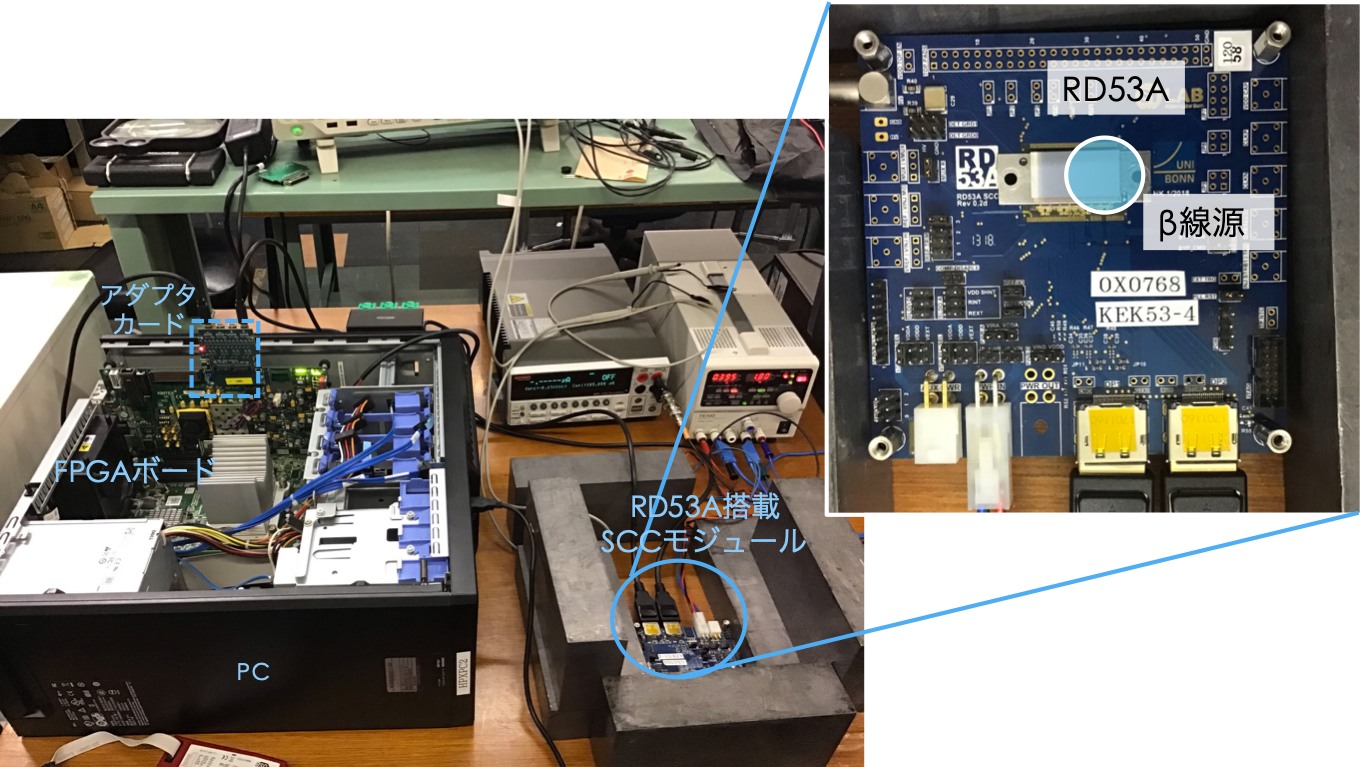
\includegraphics[width=15cm]{./figure/Setup.png}
  \caption{セットアップ}
  \label{fig:setup}
\end{figure}

\subsection*{PC}
PCからPCIeによって接続されたFPGAボードに制御コマンドを送る.また,FPGAボードからきたデータを整理する.DAQの基本的なソフトウェアとファームウェアはYARRのDAQシステムを用いた.YARRとは読み出しシステムの構築と性能向上を目指すオープンソースプロジェクトである.

\subsection*{FPGAボード}
Xilinx, Inc.のKintex-7 FPGA搭載KC705評価ボードを使用した.このFPGAボードは,研究室規模の実験で使うことを想定していることから,一般的に流通していて入手性がよいため,このFPGAボードを使用している.また,KC705はPCIe通信に対応し,PCとPCIe間では5.12 $\mathrm{Gbps}$の通信速度に対応している.今回はYARRのシステムに外部トリガを受信,処理を行う機能を追加し,RD53Aの出力するHitOR信号を用いて,外部トリガを受信できているかを確認した.

\subsection*{アダプタカード}
ASICはDP-mDPケーブルからmDP-HPCアダプタカードを通してFPGAボードに接続される.

\subsection*{RD53A搭載Single Chip Cardモジュール}
ASICを1チップ搭載した試験用モジュールがSingle Chip Cardモジュールである.今回試験したのはアップグレード用のプロトタイプ版ASICであるRD53A搭載のモジュールである.センサ付きのRD53Aが搭載されたモジュールの写真を以下に示す.
RD53Aは細い金属ワイヤにより基板上の回路パターンと電気的に接続されている.基板にRD53Aが外部と通信するためのDPコネクタ(図中:DP1),電源供給のためのmolexコネクタ(図中:PWR IN),センサに電圧を印加するためのLEMOコネクタ(図中:HV),センサが検出した信号を外部に出力するためのDPコネクタ(DP2)が実装されている.
\begin{figure}[h]
  \centering
  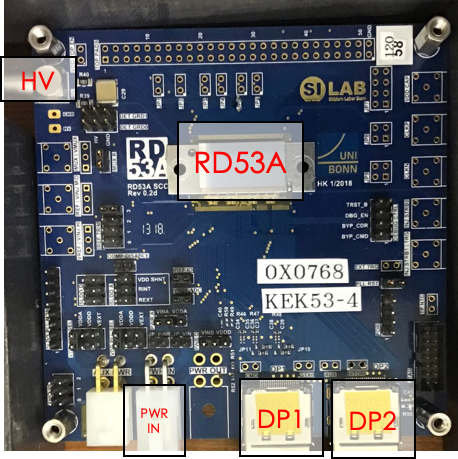
\includegraphics[width=7cm]{./figure/rd53a.png}
  \caption{センサ付きRD53A搭載Single Chip Cardモジュール}
  \label{fig:scurve}
\end{figure}

今回電源とセンサに印加した電圧は\ref{tab:voltage}に示す.

\begin{table}[h]
  \centering
  \caption{今回RD53Aとセンサに供給した電圧}
  \begin{tabular} {|l|cc|c|} \hline
     & RD53A & RD53A & ピクセル \\ 
     & アナログ回路 & デジタル回路 & センサ \\ \hline
    印加電圧[$\mathrm{V}$] & 1.80 & 1.80 & -50 \\ \hline
  \end{tabular}
  \label{tab:voltage}
\end{table}


\subsection*{$\beta$線源}
今回は粒子線として$\beta$線源であるストロンチウム90を使用した.ストロンチウム90は中性子過剰であるため,$\beta$崩壊によってイットリウム90を生成し,その後さらなる$\beta$崩壊によってジルコニウム90となる.半減期は28.79年であるが,2段階の$\beta$崩壊が起こるため,$\beta$線のエネルギーは高いものになっている.式\ref{eq:beta}にベータ崩壊の機構を,式\ref{eq:sr90}にストロンチウムの崩壊過程を示す.\par
\begin{equation}
  \label{eq:beta}
  n \rightarrow p^{+} + e^{-} + \overline{\nu_e}
\end{equation}
\begin{equation}
  \label{eq:sr90}
  \ce{^{90}Sr} \rightarrow \ce{^{90}Y} \rightarrow \ce{^{90}Zr}
\end{equation}


$\beta$線の今回用いた$\beta$線源は2017/02/13時点で$ 5.00 \times 10^3 \mathrm{Bq}$のものであった.すなわち現在の放射能は以下のように求められる.

\begin{equation}
\label{eq:radiation}
  A = -\lambda N_1 = A_0 \exp \left( - \frac{\ln 2}{T} t \right)
\end{equation}

ここで,
\begin{table}[h]
  \centering
  \begin{tabular}{cc} \hline
    $A_0$ & 2017/02/13時点での放射能($ 5.00 \times 10^3 \mathrm{Bq}$)\\
    $T$ & \ce{^{90}Sr}の半減期(28.79 $\mathrm{year}$)\\
    $t$ & 2017/02/13から現在までの時間(25/12 $\mathrm{year}$)\\ \hline
  \end{tabular}
\end{table}


式\ref{eq:radiation}より,現在の放射能$A$は,$4.76 \times 10^3 \mathrm{Bq}$と求まる.
  

%\begin{table}[h]
%  \centering
%  \caption{今回使用した$\beta$線源の放射能}
%  \begin{tabular}{|l|c|} \hline
%    基準日 & 2017/02/13 \\
%    放射能 & 5.00 $\times 10^3 \mathrm{Bq}$ \\ \hline
%  \end{tabular}
%  \label{tab:beta}
%\end{table}



\section{伝達確認}
\label{sec:scans}
ソーススキャンを行うために,既存のKC705用YARRファームウェアに外部トリガを処理する機能を追加した.本節では,機能を追加したファームが外部トリガの受信確認について述べる.

\subsection{コマンド信号とデータ信号の確認}
オシロスコープでコマンド信号とデータ信号をRD53A SCC上でプローブし,波形を確認した.

\subsection{デジタルスキャン}
全ピクセルのデジタル回路に複数回擬似パルスを注入して,注入した回数のうち何回応答が返ってくるのかを確認する.この作業をデジタルスキャンと呼ぶ.全ピクセルごとの回路の応答を確認し,データの転送線,FPGA内部の処理,PCへの通信の各経路でデータの損失がないことを確認するのに有効である.図\ref{fig:digital}に100回擬似パルスを注入した時の応答数の分布を示す.
\begin{figure}[h]
  \centering
  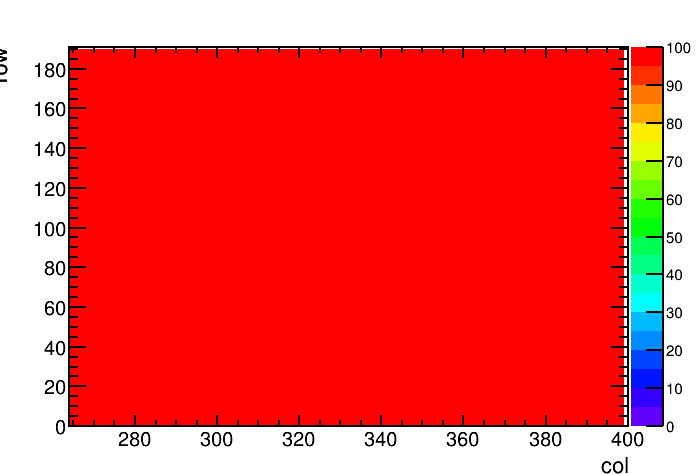
\includegraphics[width=7cm]{./figure/DigitalScan.png}
  \caption{デジタルスキャン}
  \label{fig:digital}
\end{figure}


\subsection{アナログスキャン}
アナログ回路に複数回擬似パルスを注入して,注入した回路のうち何回応答が返ってくるのかを確認した.この作業をアナログスキャンと呼ぶ.今回はDiff FEのみを使用するので,その他のフロントエンドは,グローバルレジスタの''EnCoreColSync1/2'',''EnCoreColEnLin1/2''を全て0にすることで非使用に設定した.この時,図\ref{fig:analog1}のように応答のない領域が存在した.これは,バイアスレールによりASICのプリアンプのVirtual GNDによる電位差でセンサのポリシリコン抵抗を介して電流が流れている影響だと考えられられており,Diff FEアナログ回路のLCC回路をオンにすることで改善することが知られている.本論文では,グローバルレジスタ値の''DiffLccEn''を0から1に変更し,''DiffLcc''を255にすることでLCC回路をオンにし,電圧をかけた.LCC回路をオンにした場合のアナログスキャンの様子を図\ref{fig:analog2}に示す.オフの場合と比較すると,応答のない領域が改善されているのがわかる.

\begin{figure}[h]
  \centering
  \begin{minipage}[b]{0.4\linewidth}
    \centering
    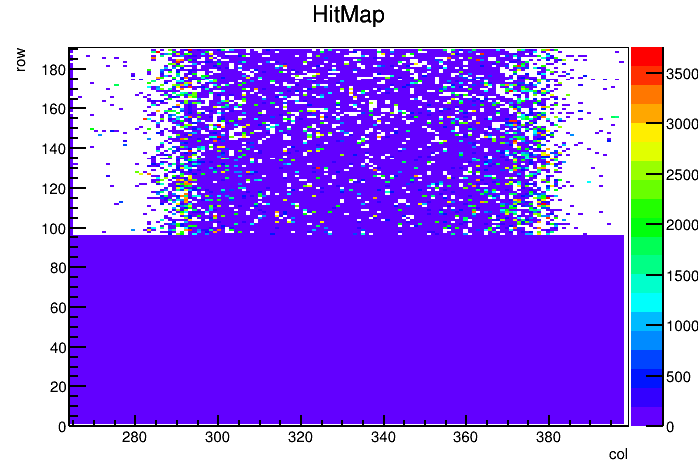
\includegraphics[width=6cm]{./figure/AnalogScan1.png}
    \subcaption{LCC回路をオフ}
    \label{fig:analog1}
  \end{minipage}
  \begin{minipage}[b]{0.4\linewidth}
    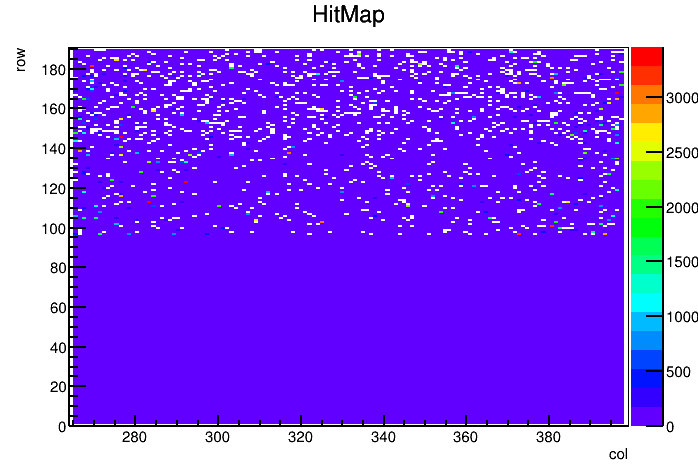
\includegraphics[width=6cm]{./figure/AnalogScan3.png}
    \subcaption{LCC回路をオン}
    \label{fig:analog2}
  \end{minipage}
  \caption{アナログスキャン}
\end{figure}


\subsection{閾値のチューニング}
\begin{figure}[h]
  \centering
  \begin{minipage}[b]{0.4\linewidth}
    \centering
    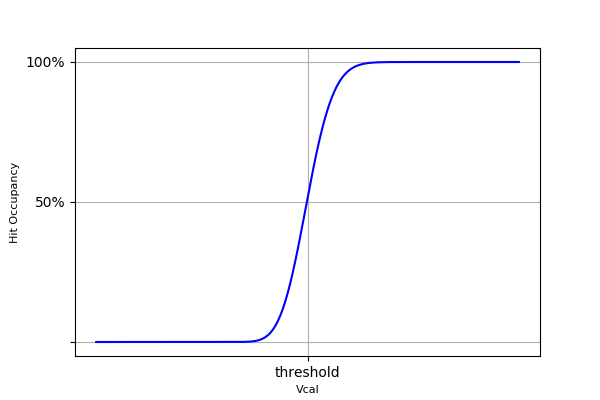
\includegraphics[width=7cm]{./figure/scurve.png}
    \subcaption{注入電荷$V_{cal}$と応答率の関係}
    \label{fig:scurve}
  \end{minipage}
  \begin{minipage}[b]{0.4\linewidth}
    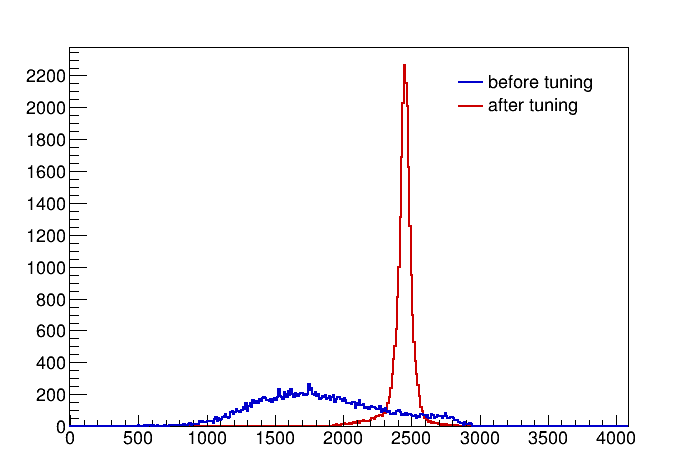
\includegraphics[width=7cm]{./figure/ThreDiff.png}
    \subcaption{チューニング前後閾値分布}
    \label{fig:ThrDistBefore}
  \end{minipage}
  \caption{閾値チューニング}
\end{figure}

閾値とはピクセルの応答率が50$\mathrm{\%}$となる電荷量で定義され,閾値が目標値になるように各ピクセルのDAC値を調節する作業を閾値のチューニングという.信号が閾値を超えたかあどうかでヒットと認識するかどうかの判定を行なっているが,信号には正規分布に従うノイズが載るため,信号がヒットとして認識される閾値には幅がある.そのため,注入電荷を変化させながら,各ピクセルに試験電荷を複数回入射したときの応答数の関係は,図\ref{fig:scurve}のような曲線になる.この曲線をSカーブと呼び,これを誤差関数でフィッティングすることで,応答率が50 $\mathrm{\%}$となる閾値を求める.
\begin{eqnarray}
  f(Q_{inj}) &=& \frac{1}{2} \left( 1 + \rm{erf} \left( \frac{Q_{inj} - Q_{thr}}{\sqrt{2} \sigma} \right) \right) \\
  \rm{erf}(x) &=& 1- \frac{2}{\sqrt{\pi}} \int^x _0 e^{-t^2} dt
  \label{eq:scurve}
\end{eqnarray}


閾値チューニング前後の各ピクセルの閾値のヒストグラムを図\ref{fig:ThrDistBefore}に示す.目標値は2400$\mathrm{e}$と設定した.2400$\mathrm{e}$という閾値は,センサの厚みとノイズ信号の大きさを考慮した値である.今回使用したセンサの厚みは,150 $\mathrm{\mu m}$であり,式\ref{eq:thr}の厚み300 $\mathrm{\mu m}$の場合のおよそ$1/2$であるため,全て空乏化した場合に発生する信号は10000 $\mathrm{e}$である.まず,この信号をASICが読み出す際に,4分割されてしまったとしても,検出してほしいために閾値は2400 $\mathrm{e}$以下であることが望ましい.また,ノイズ$\sigma$の大きさに対して6-7 $\sigma$離れている必要があるため,バイアスレール有りの場合,$\sigma = 200 \mathrm{e}$と知られているため,1200 $\mathrm{e}$以上にすることが望ましい.閾値のヒストグラムを見ると,1200 $\mathrm{e}$にチューニングした場合は,1200 $\mathrm{e}$以下まで多く分布してしまっているため,今回は分布が1200 $\mathrm{e}$以上に収まるような,2500 $\mathrm{e}$を目標値としてチューニングを行なった.

\subsection{ノイズスキャン}
任意の周波数でトリガを発行し,その全トリガ数に対するのアナログ回路から何回応答が返ってくるのかを確認する.この作業をノイズスキャンと呼ぶ.ピクセルセンサが粒子線以外の信号に対して反応していないことを確認するために有効である.\par
この作業によって,粒子線以外の信号に対して反応している部分は非使用に設定される.引き続きDiff FEのみを使用した.任意の周波数でトリガを送り,その時のアナログ回路からの応答に対して,閾値を超えるものを非使用に設定する.この作業をノイズスキャンと呼ぶ.今回は5000 $\mathrm{Hz}$で5分間ノイズスキャンを3回行なった.以下にノイズスキャンを行う前と行なった後のOccupancy MapとEnable Pixel Mapを示す.図\ref{fig:enablemap}より,非使用になっているピクセルが上半分に集中しているのが見て取れる.これは,センサ単体の試験で必要となるバイアスレールの影響であり,バイアスレールが存在すると,図\ref{fig:noisedist}のように,ノイズが増えることが知られている.

\begin{figure}[h]
  \centering
  \begin{minipage}[b]{0.45\linewidth}
    \centering
    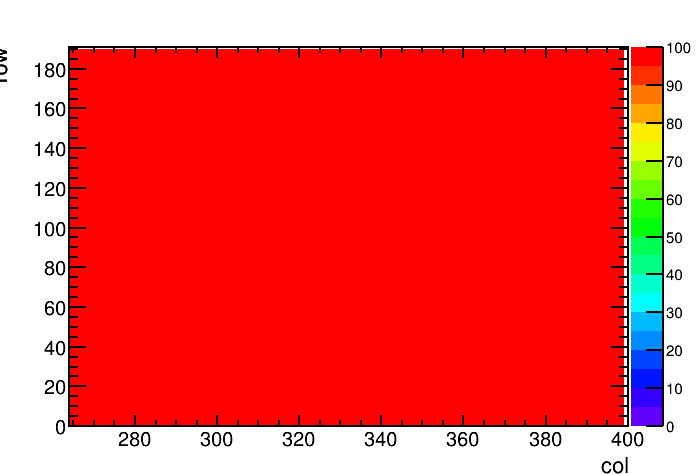
\includegraphics[width=7cm]{./figure/DigitalScan.png}
    \subcaption{ノイズスキャン前}
    \label{fig:bfnoise}
  \end{minipage}
  \begin{minipage}[b]{0.45\linewidth}
    \centering
    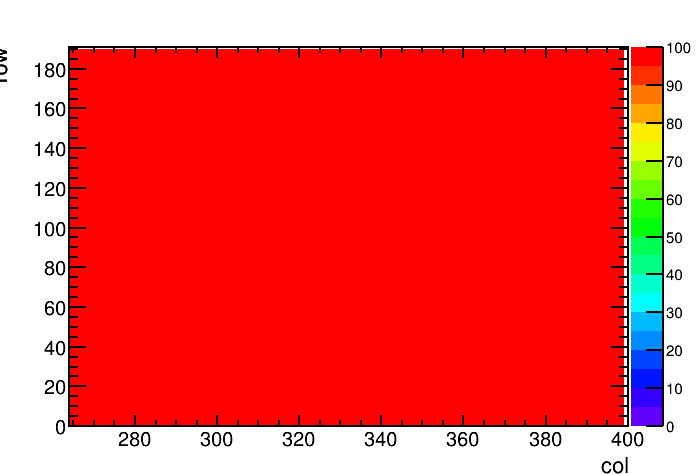
\includegraphics[width=7cm]{./figure/DigitalScan.png}
    \subcaption{ノイズスキャン後}
    \label{fig:afnoise}
  \end{minipage}
  \caption{Occupancy Map}
\end{figure}

\begin{figure}[h]
  \centering
  \begin{minipage}[b]{0.45\linewidth}
    \centering
    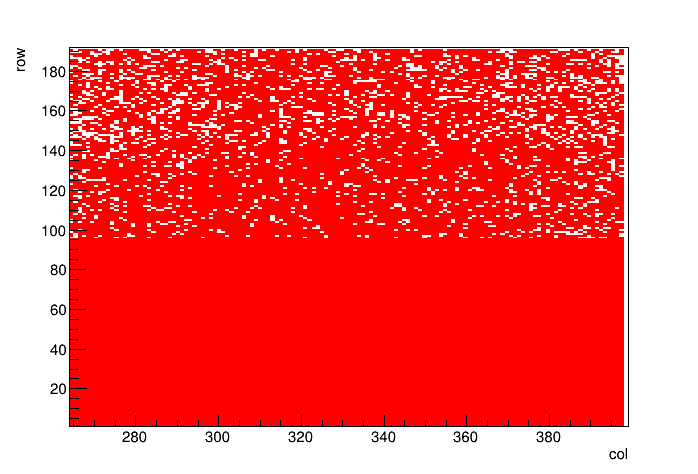
\includegraphics[width=7cm]{./figure/EnablePix.png}
    \subcaption{以降使用したピクセルの分布}
    \label{fig:enablemap}
  \end{minipage}
  \begin{minipage}[b]{0.45\linewidth}
    \centering
    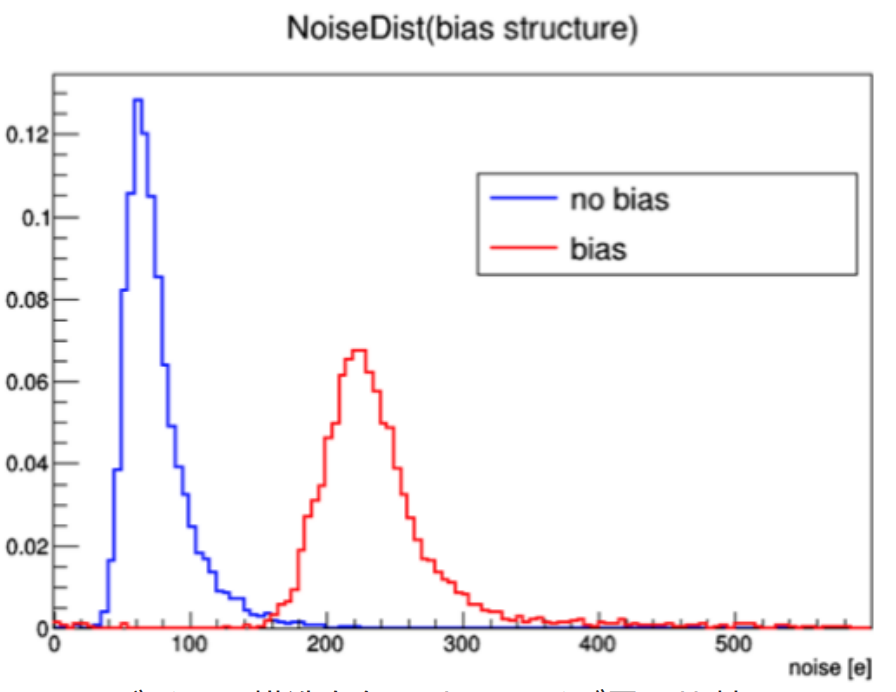
\includegraphics[width=6cm]{./figure/noisedist.png}
    \subcaption{バイアスレールの有無によるノイズ量比較}
    \label{fig:noisedist}
  \end{minipage}
  \caption{非使用なピクセルとバイアスレールによる影響}
\end{figure}


\subsection{HitOR信号の伝達確認}
モジュールの上に$\beta$線源を配置し,オシロスコープでHitOR信号をRD53A SCC上でプローブすることで,波形を確認した.また,FPGAまでHitOR信号が伝わっているかどうか,正常に処理され,そのタイミングでトリガが出力されているかどうかをVivadoのLogic Analyzerを用いて確認した.それが以下の図である.



このようにファームウェアに外部トリガを取得し,処理する機能を追加できていることを確認した.






